\documentclass{beamer}
\usetheme{metropolis}           % Use metropolis theme
\usepackage{outlines}

\title{Introducción y Conceptos básicos de bases de datos}
\date{\today}
\author{Alex Di Genova}
\institute{Universidad de O'higgins}
\begin{document}
  \maketitle
  
  
  
  \begin{frame}{Outline}
  \tableofcontents
\end{frame}

\section{Bienvenida curso de Bases de datos}
  \begin{frame}{Presentación}     
   % \begin{itemize}
\only<1>{
  Alex Di Genova
    \begin{outline}
    \1 2003--2008 Ingeniero en Bioinformatica. 
    \1 2013-2017 Doctor en Sistemas Complejos.
    \1 2017-2021 Postdoctorado en algoritmos y cancer (Francia).
    \1 2022 - Profesor Asistente UOH.
    \2 Di Genoma Lab 
    	\3 Combinamos el desarrollo de nuevos algoritmos, análisis de genomas y tecnologías ómicas de última generación para estudiar sistemas biológicos complejos.
    \end{outline}
   }
   
   \only<2>{
   \begin{figure}
  \centering
    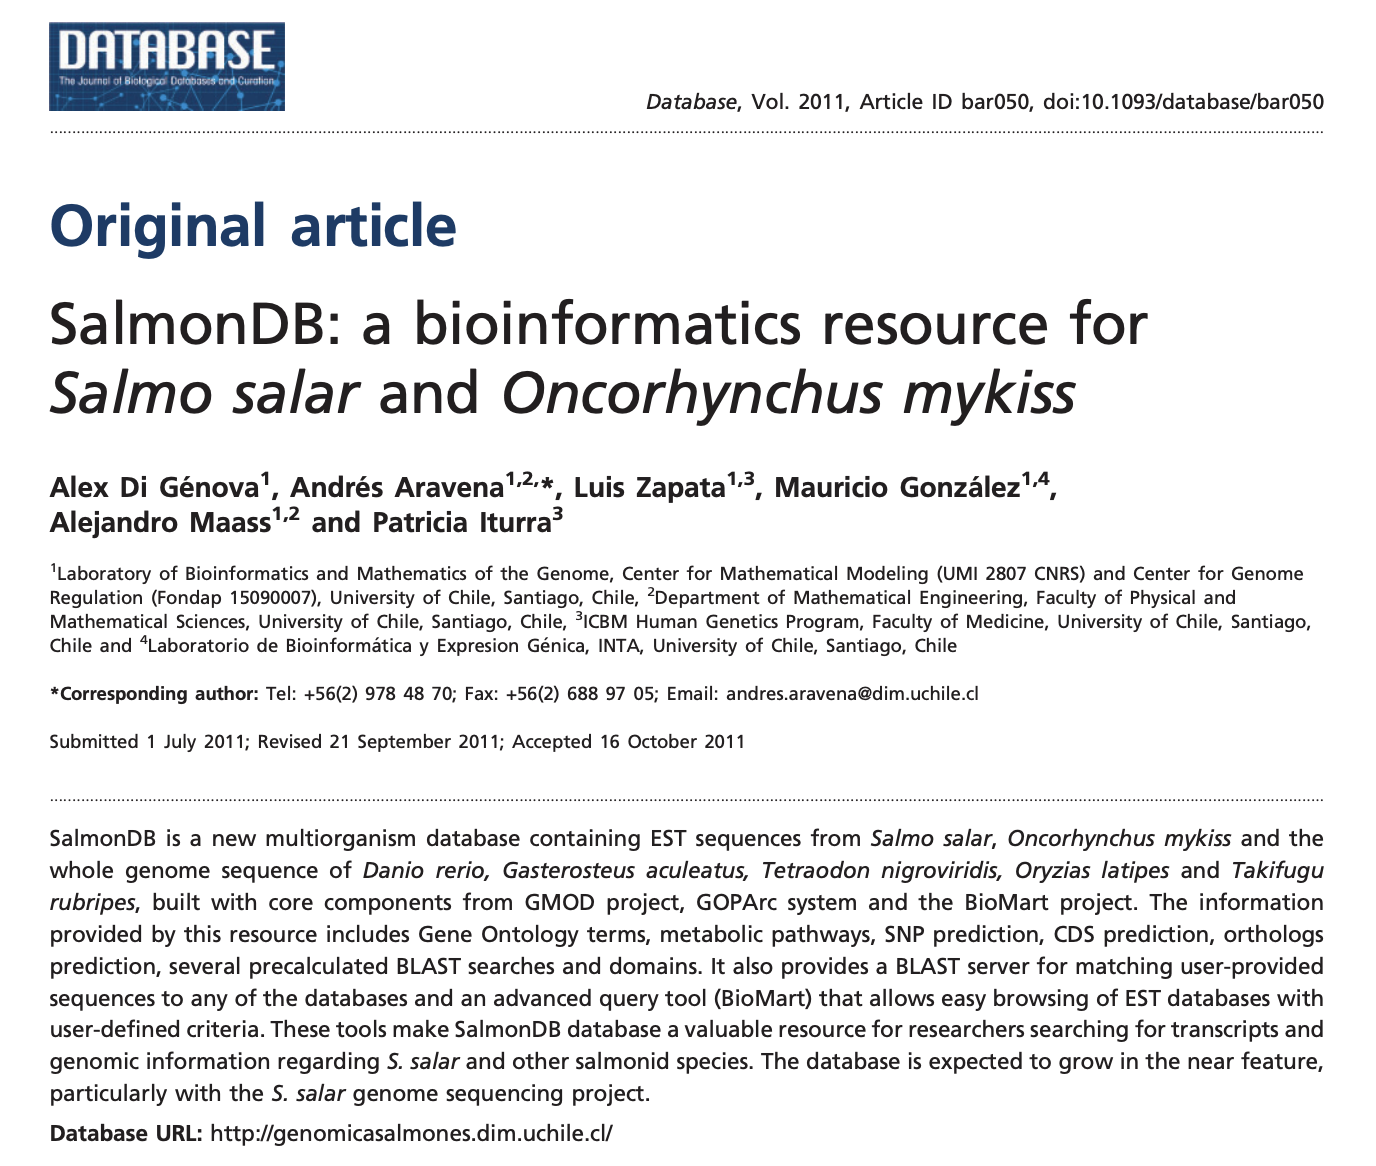
\includegraphics[scale=0.4]{img/salmondb.png}
 \end{figure}
   } 
   \only<3>{
   \centering
   \Large
   Alumnas y Alumnos
   }
  \end{frame}
 
 
  \section{Planificación curso BD}
  \begin{frame}{Unidades}
  \only<1>{
    \begin{itemize}
    	\item 4 Unidades (14 semanas)
		\begin{itemize}
			\item Modelamiento de bases de datos (3 semans)
			\item Modelo Relacional (4 semanas)
			\item Lenguaje de Consulta SQL (3 semanas) 
			\item Transacciones y Bases de datos no relacionales (4 semanas)
		\end{itemize}
	  \end{itemize}
}
 \only<2>{
Modelamiento de bases de datos 
\begin{itemize}
\item \emph{Cada \textbf{persona} puede habitar en solo una \textbf{vivienda} y estar registrada en solo un \textbf{municipio} pero pude ser propietaria de varias viviendas.} \dots
\item La empresa está organizada en departamentos. Cada uno tiene un nombre único, un número único y un empleado concreto que lo administra. Un departamento controla una cierta cantidad de proyectos, cada uno de los cuales tiene un nombre único, un número único y una sola ubicación.
\end{itemize}
}
\only<3>{
Esquema Relacional 
\begin{figure}
  \centering
    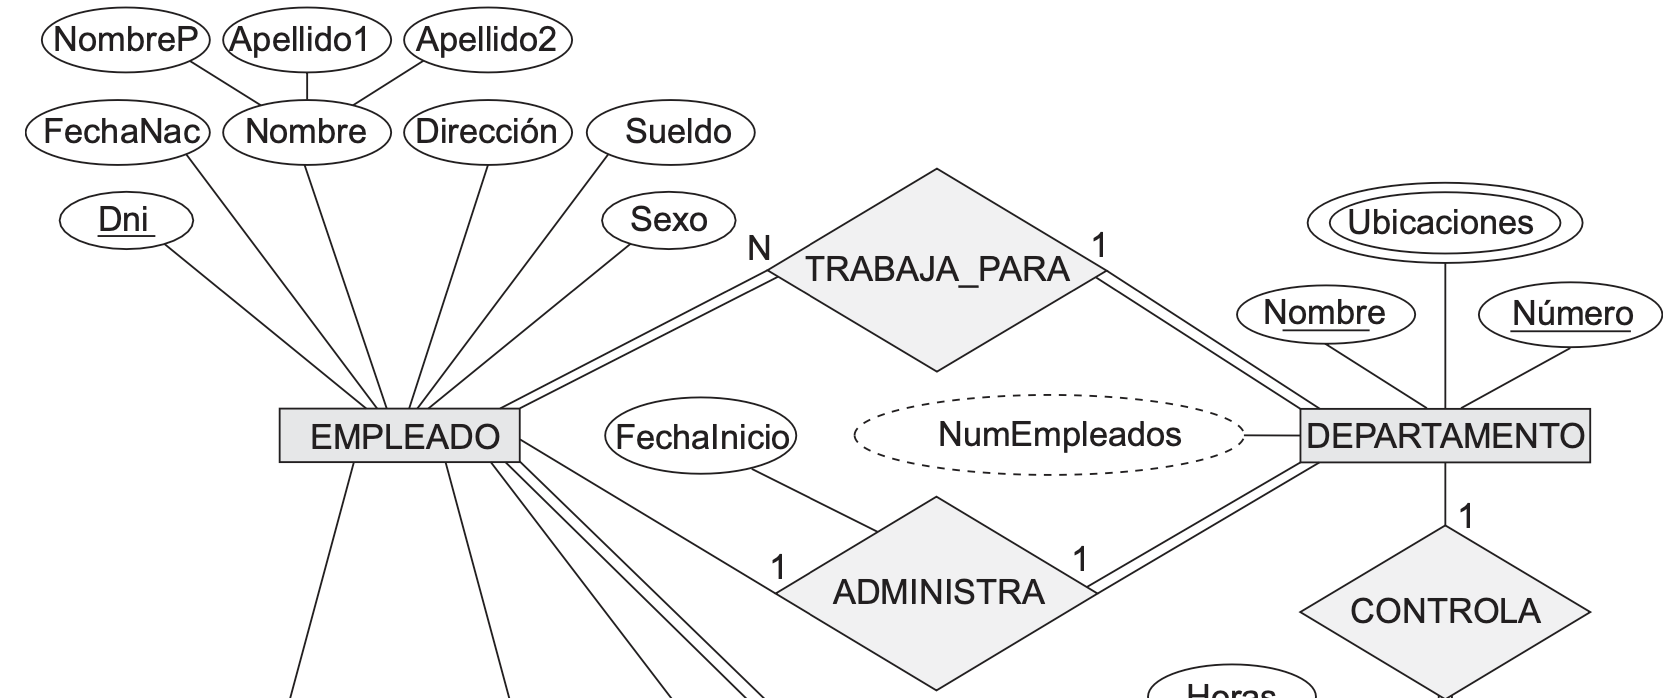
\includegraphics[scale=0.4]{img/er.png}
 \end{figure}
}
\only<4>{
Diagrama Entidad-Relacion (Modelo UML)
\begin{figure}
  \centering
    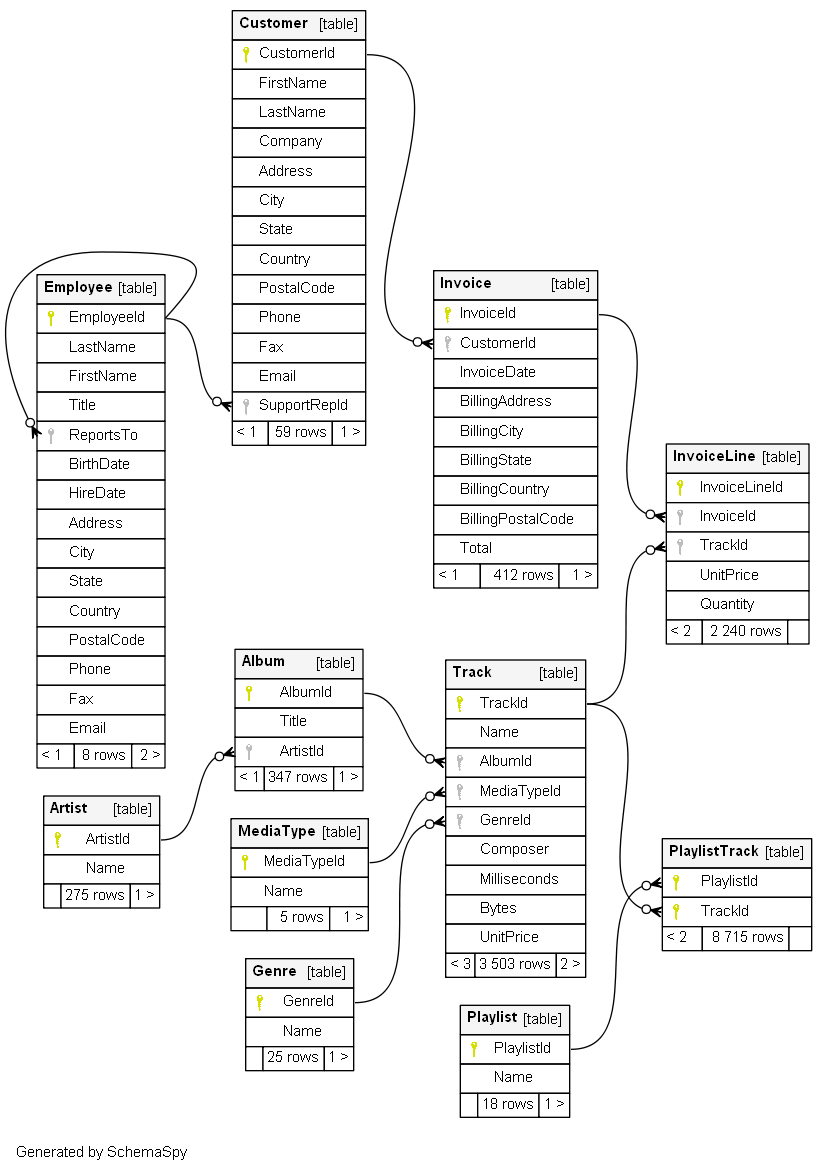
\includegraphics[scale=0.2]{img/db-uml.png}
 \end{figure}
}
\only<5>{

SQL (SQLite3)
\begin{figure}
  \centering
    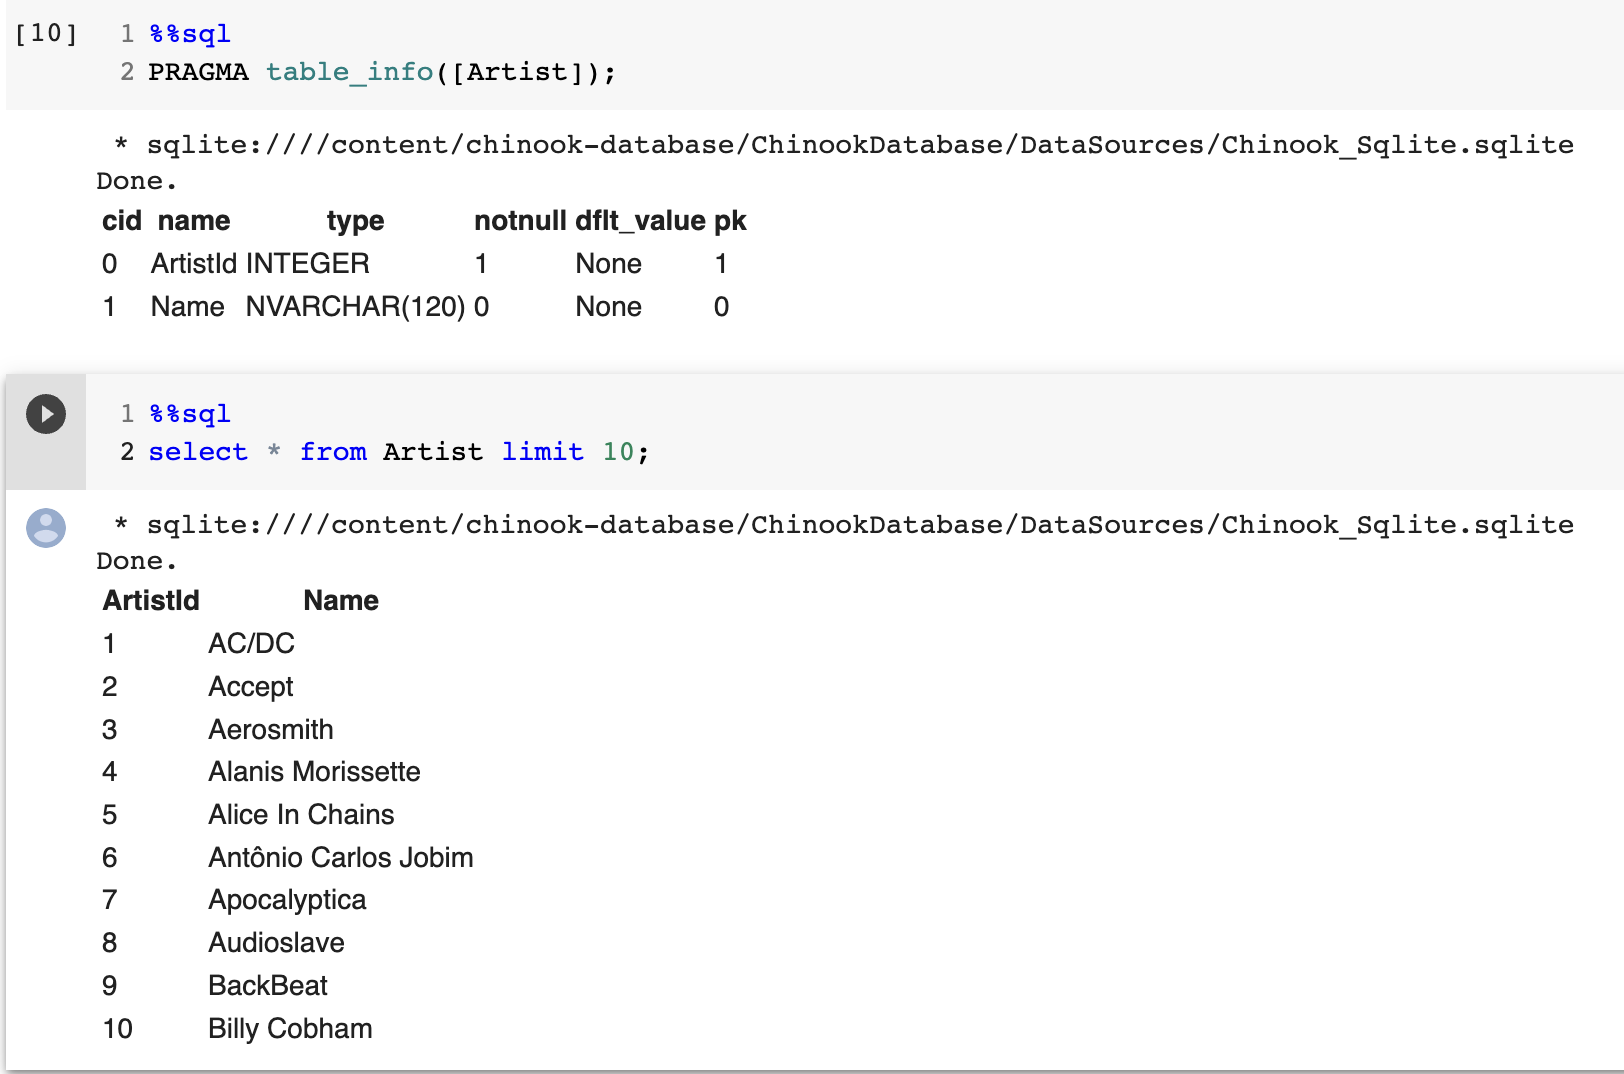
\includegraphics[scale=0.3]{img/sql-ex.png}
 \end{figure}
 
 GoogleColab -- \url{https://colab.research.google.com/}
 
  \href{https://www.youtube.com/watch?v=8VFYs3Ot_aA&t=115s}{Video descriptivo de GoogleColab}

}
\only<6>{
Transacciones
\begin{itemize}
\item Atomicidad
\item Conservación de la consistencia.
\item Aislamiento
\item Durabilidad
\end{itemize}
	\begin{figure}
  \centering
    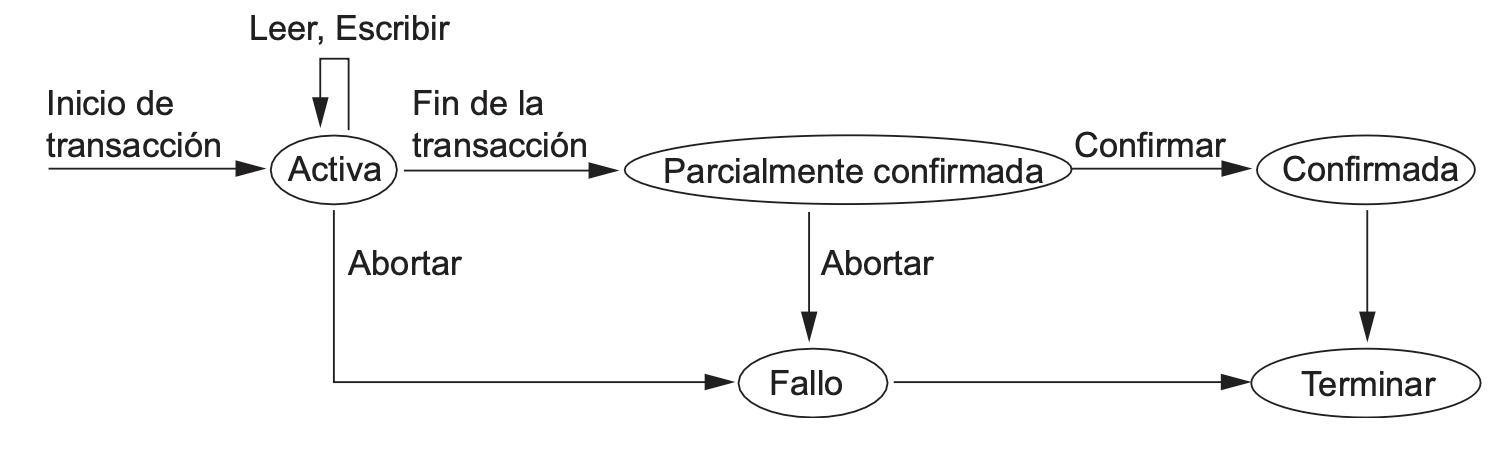
\includegraphics[scale=0.3]{img/transacciones.png}
 \end{figure}
 No-SQL
 \begin{itemize}
\item levelDB, rocksDB \dots
 \end{itemize}
}
%Las transacciones deben poseer varias propiedades, a menudo denominadas propiedades ACID, que deben ser implementadas por el control de la concurrencia y los métodos de recuperación del DBMS. Las propiedades ACID son las siguientes:
% Atomicidad. Una transacción es una unidad atómica de procesamiento; o se ejecuta en su totalidad o no se ejecuta en absoluto.
% Conservación de la consistencia. Una transacción está conservando la consistencia si su ejecución completa lleva a la base de datos de un estado consistente a otro.
% Aislamiento. Una transacción debe aparecer como si estuviera ejecutándose de forma aislada a las demás. Es decir, la ejecución de una transacción no debe interferir con la ejecución de ninguna otra transacción simultánea.
% Durabilidad. Los cambios aplicados a la base de datos por una transacción confirmada deben persis- tir en la base de datos. Estos cambios no deben perderse por culpa de un fallo.

  \end{frame}
  
  \begin{frame}{Evaluaciones}
  \begin{outline}
  	
  	\1 Controles :
	\2 Control 1:  Semana del 9 Mayo.
	\2 Control 2:  Semana del 13 Junio.
	\2 Control 3:  Semana del 11 Julio.
	\uncover<2->{
	\1 Tareas:
	\2 Tarea 1: Semana del 9 Mayo.
	\2 Tarea 2: Semana del 6 Junio. }
  \end{outline}
  \end{frame}
  
  \begin{frame}{Condiciones y Políticas de Evaluación}
  \small
  \begin{outline}
   \1 El promedio de actividades complementarias se considerará como un cuarto control (control IV) y tendrá una ponderación de 15\%. El promedio de controles I,II,III y IV con sus respectivas ponderaciones corresponderán a la nota final del curso. El curso será aprobado con una nota promedio igual o superior a 4,0.
    
 \uncover<2->{   \1 Estudiantes que se ausenten a un control tendrán la oportunidad de recuperarlo durante el periodo correspondiente al final del semestre. El control recuperativo es de carácter \textbf{acumulativo}, por lo tanto, contendrá contenido de las cuatro unidades del curso. Adicionalmente, alumnos que quieran remplazar una calificación en un control o actividades complementarias, también podrán rendir el control recuperativo.}
    
   \uncover<3->{ \1 Un/a estudiante que cometa plagio sobtendrá un 1,0 en la evaluación y el caso será informado a Escuela de Ingeniería.}
\end{outline}

  \end{frame}
  
  \begin{frame}{Resultados de Aprendizaje}
  	\begin{outline}
		\1 Diseñar diagramas de Entidad/Relacional para satisfacer las necesidades de un problema enunciado.
		\1  Realizar a partir de un diagrama Entidad/Relación un diseño relacional.
		\1 Normalizar un diseño relacional de bases de datos.
		\1 Formular consultas de distinto tipo en SQL.
		\1 Reconocer la noción de transacción y operar el sistema de recuperación de un sistema de administración de bases de datos.
		\1 Conocer sistemas de bases de datos no relacionales.
	\end{outline}
  \end{frame}
  
\end{document}